\clearpage
\subsubsection{x86 + MSVC + \olly}
\index{\olly}
\index{x86!\Registers!\Flags}

\RU{Если попробовать этот пример в \olly, можно увидеть, как выставляются флаги}\EN{We
can see how flags are set by running this example in \olly}.
\RU{Начнем с ф-ции}\EN{Let's begin with} \TT{f\_unsigned()}\RU{, которая работает с беззнаковыми числами}
\EN{ function, which works with unsigned number}.
\RU{В целом, в каждой ф-ции, \CMP исполняется три раза, но для одних и тех же аргументов, так что
флаги будут три раза одни и те же каждый раз}\EN{\CMP executed thrice here, but for the same arguments, so
flags will be the same each time}.

\RU{Результат первого сравнения}\EN{First comparison results}:

\begin{figure}[H]
\centering
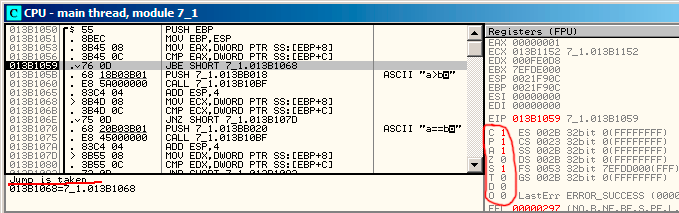
\includegraphics[scale=\FigScale]{patterns/07_jcc/simple/olly_unsigned1.png}
\caption{\olly: \TT{f\_unsigned()}: \RU{первый условный переход}\EN{first conditional jump}}
\label{fig:jcc_olly_unsigned_1}
\end{figure}

\RU{Итак, флаги}\EN{So, the flags are}: C=1, P=1, A=1, Z=0, S=1, T=0, D=0, O=0.
\RU{Для краткости, в \olly флаги называются только одной буквой.}
\EN{Flags are named by one character for brevity in \olly.}

\olly \RU{подсказывает, что первый переход}\EN{gives a hint that} (\JBE) \RU{сработает}\EN{jump will be triggered}.
\RU{Действительно, если заглянуть в}\EN{Indeed, if to take a look into} \cite{Intel}, 
\RU{прочитаем там, что}\EN{we will read there that} \JBE \RU{срабатывает в случаях если}\EN{will trigger if} 
CF=1 \OrENRU ZF=1.
\RU{Условие здесь выполняется, так что переход срабатывает}\EN{Condition is true here, so jump is triggered}.

\clearpage
\RU{Следующий переход}\EN{The next conditional jump}:

\begin{figure}[H]
\centering
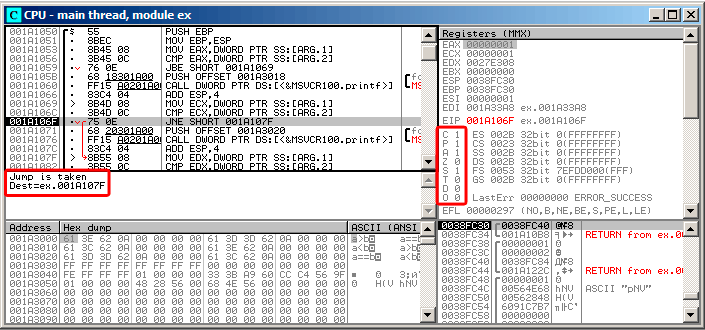
\includegraphics[scale=\FigScale]{patterns/07_jcc/simple/olly_unsigned2.png}
\caption{\olly: \TT{f\_unsigned()}: \RU{второй условный переход}\EN{second conditional jump}}
\label{fig:jcc_olly_unsigned_2}
\end{figure}

\olly \RU{подсказывает, что}\EN{gives a hint that} \JNZ \RU{сработает}\EN{will trigger}.
\RU{Действительно}\EN{Indeed}, \JNZ \RU{срабатывает если}\EN{will trigger if} ZF=0 (zero flag).

\clearpage
\RU{Третий переход}\EN{The third conditional jump} \JNB:

\begin{figure}[H]
\centering
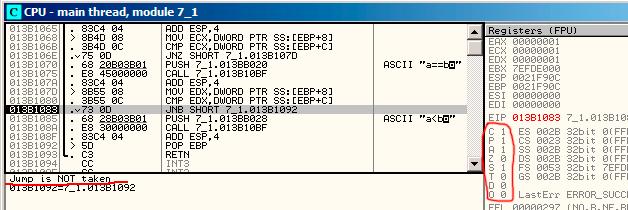
\includegraphics[scale=\FigScale]{patterns/07_jcc/simple/olly_unsigned3.png}
\caption{\olly: \TT{f\_unsigned()}: \RU{третий условный переход}\EN{third conditional jump}}
\label{fig:jcc_olly_unsigned_3}
\end{figure}

\RU{В}\EN{In} \cite{Intel} \RU{мы можем найти что}\EN{we may find that} \JNB \RU{срабатывает если}
\EN{will trigger if} CF=0 (carry flag).
\RU{В нашем случае это не так, так что переход не срабатывает, и исполняется третий по счету}
\EN{It's not true in our case, so the third} \printf\EN{ will execute}.

\clearpage
\RU{Теперь можно попробовать в \olly ф-цию}\EN{Now we can try in \olly the} \TT{f\_signed()} 
\RU{работающую с знаковыми величинами}\EN{function, which works with signed values}.

\RU{Флаги выставляются точно так же}\EN{Flags are set in the same way}: 
C=1, P=1, A=1, Z=0, S=1, T=0, D=0, O=0.

\RU{Первый переход}\EN{The first conditional jump} \JLE \RU{сработает}\EN{will trigger}:

\begin{figure}[H]
\centering
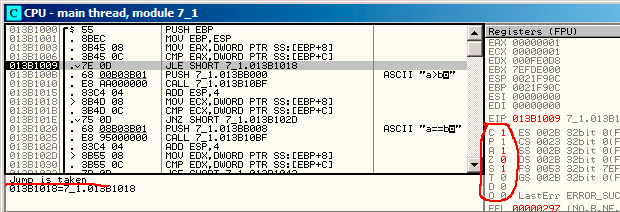
\includegraphics[scale=\FigScale]{patterns/07_jcc/simple/olly_signed1.png}
\caption{\olly: \TT{f\_unsigned()}: \RU{первый условный переход}\EN{first conditional jump}}
\label{fig:jcc_olly_signed_1}
\end{figure}

\RU{В}\EN{In} \cite{Intel} \RU{мы можем прочитать что эта инструкция срабатывает если}\EN{we may find
that this instruction is triggering if} 
ZF=1 \OrENRU SF$\neq$OF.
\RU{В нашем случае, }SF$\neq$OF\RU{, так что переход срабатывает}\EN{ in our case, so jump is triggering}.

\clearpage
\RU{Второй переход}\EN{The next} \JNZ \RU{сработает}\EN{conditional jump will trigger}: 
\RU{он срабатывает если}\EN{it does if} ZF=0 (zero flag):

\begin{figure}[H]
\centering
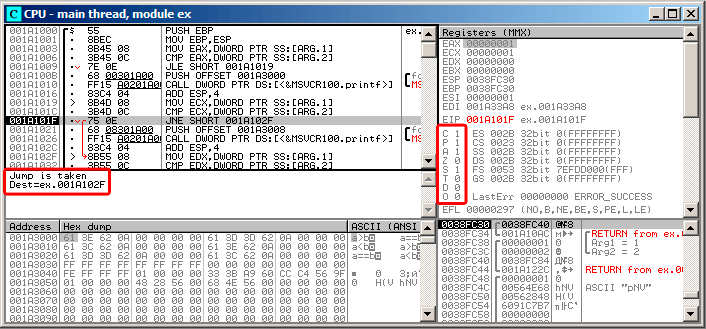
\includegraphics[scale=\FigScale]{patterns/07_jcc/simple/olly_signed2.png}
\caption{\olly: \TT{f\_unsigned()}: \RU{второй условный переход}\EN{second conditional jump}}
\label{fig:jcc_olly_signed_2}
\end{figure}

\clearpage
\RU{Третий переход}\EN{The third conditional jump} \JGE 
\RU{не сработает, потому что он срабатывает только если}\EN{will not trigger because it will only if} SF=OF, 
\RU{что в нашем случае не так}\EN{and that is not true in our case}:

\begin{figure}[H]
\centering
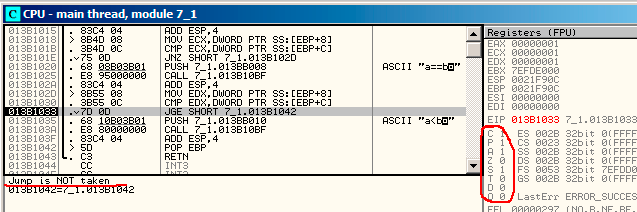
\includegraphics[scale=\FigScale]{patterns/07_jcc/simple/olly_signed3.png}
\caption{\olly: \TT{f\_unsigned()}: \RU{третий условный переход}\EN{third conditional jump}}
\label{fig:jcc_olly_signed_3}
\end{figure}
